% !TEX TS-program = pdflatex
% !TEX encoding = UTF-8 Unicode

% This is a simple template for a LaTeX document using the "article" class.
% See "book", "report", "letter" for other types of document.

\documentclass[11pt]{article} % use larger type; default would be 10pt

\usepackage[utf8]{inputenc} % set input encoding (not needed with XeLaTeX)

%%% Examples of Article customizations
% These packages are optional, depending whether you want the features they provide.
% See the LaTeX Companion or other references for full information.

%%% PAGE DIMENSIONS
\usepackage{geometry} % to change the page dimensions
\geometry{letterpaper} % or letterpaper (US) or a5paper or....
 \geometry{margin=1in} % for example, change the margins to 2 inches all round
% \geometry{landscape} % set up the page for landscape
%   read geometry.pdf for detailed page layout information

\usepackage{graphicx} % support the \includegraphics command and options
\graphicspath{ {images/} }

\usepackage{pdfpages}
\pdfminorversion=7

\usepackage{hyperref}
\hypersetup{
    colorlinks=true,
    linkcolor=blue,
    filecolor=magenta,      
    urlcolor=cyan,
}
 
\urlstyle{same}


% \usepackage[parfill]{parskip} % Activate to begin paragraphs with an empty line rather than an indent

%%% PACKAGES
\usepackage{booktabs} % for much better looking tables
\usepackage{array} % for better arrays (eg matrices) in maths
\usepackage{paralist} % very flexible & customisable lists (eg. enumerate/itemize, etc.)
\usepackage{verbatim} % adds environment for commenting out blocks of text & for better verbatim
\usepackage{subfig} % make it possible to include more than one captioned figure/table in a single float
% These packages are all incorporated in the memoir class to one degree or another...

%%% HEADERS & FOOTERS
\usepackage{fancyhdr} % This should be set AFTER setting up the page geometry
\pagestyle{fancy} % options: empty , plain , fancy
\renewcommand{\headrulewidth}{0pt} % customise the layout...☺
\lhead{}\chead{}\rhead{}
\lfoot{}\cfoot{\thepage}\rfoot{}

%%% SECTION TITLE APPEARANCE
\usepackage{sectsty}
\allsectionsfont{\sffamily\mdseries\upshape} % (See the fntguide.pdf for font help)
% (This matches ConTeXt defaults)

%%% ToC (table of contents) APPEARANCE
\usepackage[nottoc,notlof,notlot]{tocbibind} % Put the bibliography in the ToC
\usepackage[titles,subfigure]{tocloft} % Alter the style of the Table of Contents
\renewcommand{\cftsecfont}{\rmfamily\mdseries\upshape}
\renewcommand{\cftsecpagefont}{\rmfamily\mdseries\upshape} % No bold!

%%% END Article customizations


%%% The "real" document content comes below...

\title{Cryptocurrency Portfolio Optimization\\
\large Decision Analytics:  Final Project - Group 6}
\author{Austin Harrison, Tine Hutchison, Michael Kennedy}
%\date{} % Activate to display a given date or no date (if empty),
         % otherwise the current date is printed 

%\usepackage{setspace}
%\doublespacing

\setlength{\parskip}{0.5em}


\begin{document}
\maketitle


\section{Abstract}

This paper presents an exploration of portfolio maximization modelling techniques and their application to cryptocurrencies in 2018 and beyond.  Using a 365 day sample of daily returns for 10 cryptocurrencies the authors conduct a computational experiment leveraging mathematical models originally developed by Harry Markowitz and William Sharpe.  Analysis of the experiment’s results and findings is complemented by a literature review of modern methods that build upon the foundation of Markowitz and Sharpe to produce results that are superior and or more reliable.

\subsection{Key Words}

Portfolio optimization; Cryptocurrency; Minimax; Finance;

\section{Introduction}

The authors seek stable investment returns that exceed that which they might find in a professionally managed fund. Supposing a light Efficient Market Hypothesis, the authors will implement a version of the Portfolio Optimization technique first proposed by Harry Markowitz in his\emph{ The Journal of Finance} article from March of 1952. At the time, Mr. Markowitz phrased his motivation, supposing that\emph{ ``...the investor does (or should) consider expected return a desirable thing and variance of return an undesirable thing”}. \cite{markowitz}

``Diversification” is a conventional response to a desire to reduce risk. Diversification is accomplished by selecting a variety of security types (stocks, bonds, real estate, etc.) from a variety of industries. Markowitz maintains that Diversification is not enough, writing \emph{``The returns from securities are too intercorrelated. Diversification cannot eliminate all variance.”}  \cite{markowitz} We see this with general market downturns, where almost the entire market will collapse at the same time. Markowitz’s method looks to identify a more truly diverse combination of holdings, going beyond simplistic diversification.

Our problem is a simple one:\emph{ How can we structure a securities portfolio that provides a reliable expected return over a long period of time?} We will examine this question in the context of the modern era, applying the technique to a selection of cryptocurrencies (BTC ETH DASH XRP LTC XLM REP XMR ETC MAID) and validating our models by applying them to a selection of stocks from the S\&P 500 Index. In both cases, we’ll be looking for a mix of elements that provides the least variance and the greatest expected return. 

\section{Literature Review}

We reviewed a variety of journal articles related to this topic, starting with Markowitz in 1952, and ending with an article on Neural Network Optimization that was published in January of 2018. The articles tend to be improving on Markowitz’s initial proposal. The first article of note is from William F. Sharpe in 1971. He explains that the quadratic formulation for Variance proposed by Markowitz is computationally expensive, and he proposes a method for approximating the variance curve with a series of segments. He writes: ‘‘if the essence of the portfolio analysis problem could be adequately captured in a form suitable for linear programming methods, the prospect for practical application would be greatly enhanced.”  \cite{sharpe71}

The Markowitz visualization (below, left) and the Sharpe visualization (below, right).

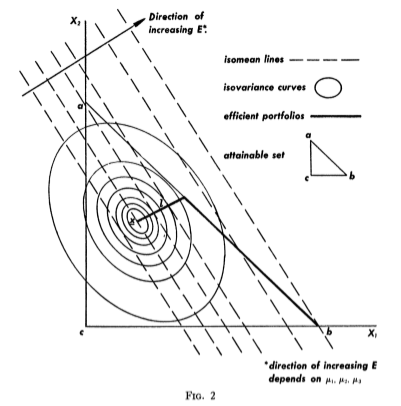
\includegraphics[width=0.5\textwidth]{mark1}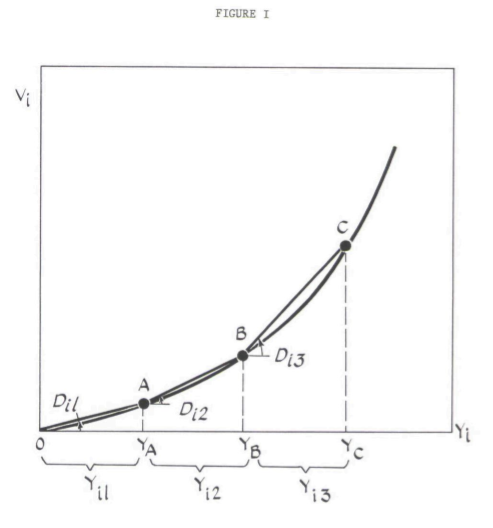
\includegraphics[width=0.5\textwidth]{sharpe1}
    
Following Sharpe in 1971, a major change in the approach was not made until 1998, when Martin Young proposed a minimax approach that looked at historical returns, instead of variance, as a shortcut to the quadratic mean-variance approach proposed by Markowitz. ``The optimal portfolio is defined as that one that would minimize the maximum loss (in dollars) over all past historical periods, subject to a restriction on the minimum acceptable average return across all observed time periods. This principle leads to portfolio selections similar to those obtained by the mean-variance selection rule of Markowitz…” \cite{young}

Young goes on to write: ``The reason mean-variance analysis fails in this setting is that what one truly wishes to achieve in a risk-averse portfolio selection rule is the avoidance of low returns, whereas mean-variance selection penalizes variation even among high returns.” This seems a strong argument in favor of his approach.

From Young in 1998, we skip ahead to Polak, et al. in 2010 (and past other influential papers). They also chose a minimax approach, building off of Young’s work. Polak’s article was possibly most useful for its exhaustive Literature review, which likely serves as a better example than our own, at least through the time of its publication.

An article from Christine Gregory, et al, in 2011 introduced us to the concept of optimizing for ``Robustness” \cite{gregory} , although this was not her innovation. Robustness addresses the problem of assuming a static $\mu$ and $\sigma$ in the Markowitz model. This boils down to setting a range of possible values for $\mu$ and $\sigma$ and optimizing from there.

Gregory, et al, also allude to min-regret models, something that she does not elaborate on. The final article we looked at for linear optimization approaches, by Xidonas, et al, in 2017, expands on this concept, calling it ``minimax regret”, where ``Regret is actually the deviation of an obtained solution from the optimum solution according to a specific scenario of parameters." \cite{xidonas}

In addition to Markowitz inspired approaches, we looked at Neural Network approaches to portfolio optimization. Specifically, we looked at an approach taken by Zhao, et al, in their article published in January of 2018. In the article, the authors talk about the observed imbalance in correlation among stocks, depending on the overall direction of the market. Specifically: ``It is a stylized fact that equity returns are more correlated during market downturns than market upturns… This characteristic, known as asymmetric dependence, violates the assumption of modern portfolio theory that the financial returns follow joint normal distributions and their dependence can be fully described by the linear correlation coefficient as suggested by Markowitz (1952).” \cite{zhao} They suggest that models built with this assumption built in, that are able to utilize short selling, can outperform other models. The statistical concept in play here is a ‘copula’, which is a multivariate probability distribution. They compare the results of various optimization approaches, with and without Neural Networks, with weekly rebalancing. The results are, as they write, ``clearly superior”, and worth sharing here:

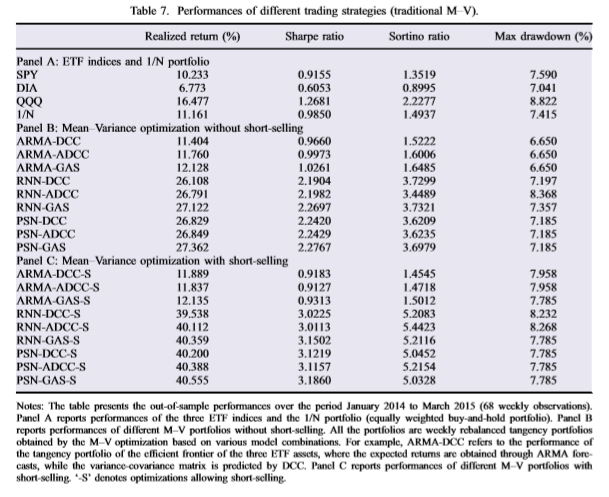
\includegraphics[width=\textwidth]{table1}

 
\section{Methodology}

Our primary objective is to determine an optimal combination of financial assets that offers minimal risk while achieving the maximum return at that level of risk. Our method of doing so will follow Markowitz’s methodology to determine the efficient frontier of investment portfolios of a given set of financial assets. From there, we will also incorporate the Sharpe Ratio \cite{sharpe66} as an indicator to determine a good risk-return tradeoff.

\subsection{Assumptions}

The methods used assume that future financial performance is indicated by past performance. Though this historically holds true on an aggregate level, there is no guarantee that future performance will follow past trends. 

A risk-free rate of zero was used for the Sharpe Ratio. We could have used a rate for an alternative baseline investment option, such as the long-term yield on the US Treasury coupon bonds. Since the focus of our study was optimization, zero was chosen to reduce the number of variables as the various choices of risk-free rates could significantly changes the results.

\subsection{Model Formulation}

For a Markowitz model the objective is to minimize the overall variance for the portfolio.  The function for that variance is equal to the summation of the product of the weights for each combination of cryptocurrency pairs multiplied by the covariance of each pair.  The scientific notation for that objective function is typically presented as such. 

\begin{equation} 
\mu_p^2  = \sum_i \sum_j w_i w_j \sigma_{ij}
\end{equation}

That objective is subject to the following constraints.  First, the total return for the portfolio, equal to the sum of the weight for each currency in the portfolio multiplied by its expected return is given an overall expected value.  The notation for that function can be represented by the following.

\begin{equation} 
E(R_p) = \sum_i w_i E(R_i)
\end{equation}
 
For the model presented here, we set that constraint equal to the average return for all ten currencies over the last 365 days. In doing so, we have ensured that the return expected from an optimized portfolio is at least as good as a portfolio selected with equal amounts invested in each currency.
 
The next constraint applied ensures that the sum of the decision variables, the cryptocurrency weights, equals 100\%.  That constraint can be represented by the following function

\begin{equation} 
\sum_i w_i = 1
\end{equation}
 
Lastly, the weight selected for each cryptocurrency in our portfolio had to be greater than or equal to 0 $(wi , wj >= 0)$.  For the optimization of stock portfolios that permit short selling it can be beneficial to allow weights $<0$, but for the problem at hand 0 was set as a lower boundary. 

\subsection{Performance Evaluation}

The performance of our model can be assessed by comparing an optimized portfolio’s performance against a similar existing portfolios performance as a benchmark. As there are few cryptocurrency portfolios currently being traded, we chose to apply our portfolio optimization model to a subset of S\&P 500 companies and compare the performance to an S\&P 500 index fund. The resulting optimized portfolio should have similar expected performance as the index fund over the same period.  

\section{Computational Experiment and Results}

\subsection{Data}

Historical cryptocurrency data was gathered in Python using the CryptoCompare API. This data included the currency exchange rate to USD as of 00:00 UTC everyday between 3/12/2017 and 3/11/2018. 

Historical data for the S\&P 500 model validation analysis was gathered from random subsets of companies in the S\&P 500 from Google Finance using the pandas\_datareader module in Python. This data included daily closing prices from 1/1/2015 through 3/11/2018.

The Python script used to download both the cryptocurrency and stock data was written to be easily modified to change the currencies or stocks and the date ranges to analyze for future optimizations.

\subsection{Simulations}

Prior to building an optimization model, simulations of random portfolios were run. This simplified approach gave a reasonable estimate of the kinds of values we could expect from the optimized model. The figure below shows the results of 10,000 randomly weighted portfolios. The random numbers were drawn from a uniform distribution.


\begin{figure}[h]
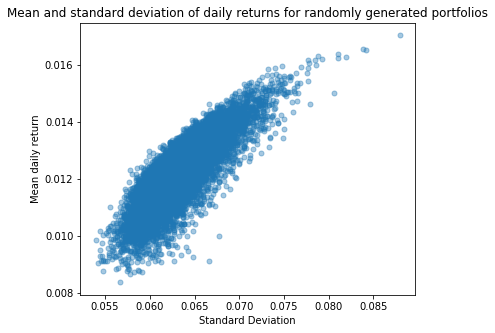
\includegraphics{sim1}
\centering
\end{figure}
 
\section{Model}

The optimization model was created using the Gurobi Python interface. Following the model formulation, the decision variables were the weights of each cryptocurrency in the portfolio with the constraint that the total of the weights must equal one. An initial optimization was performed using these constraints to give the weights that provided the minimum variance. Following this, an additional constraint to set the target portfolio return was added and a number of models were run by changing the target return from the minimum to maximum returns. This provided an efficient frontier showing the minimum risk at the varying levels of return.

While the model was optimized through the varying levels of target return, the Sharpe Ratio of each optimized portfolio was calculated and recorded. The Sharpe Ratio provides a way to reasonably estimate a good tradeoff between risk and return, where return is higher than the return given for the minimum risk portfolio. 

\section{Results}

\subsection{Cryptocurrency}

The figure below shows the results of the simulations and Gurobi optimization model. The orange dots are the 10,000 simulated portfolios with randomly assigned weights of the decision variables. The green curve shows the efficient frontier with points for the minimum risk portfolio and the maximum optimized Sharpe Ratio portfolio. The minimum risk portfolio is estimated to provide a daily return of 0.8\% with a volatility (standard deviation) of 0.04. The maximum Sharpe ratio portfolio is estimated to give 1.1\% daily return with volatility of 0.053. The allocations of cryptocurrencies and weights for the two optimized portfolios are shown in the appendix.

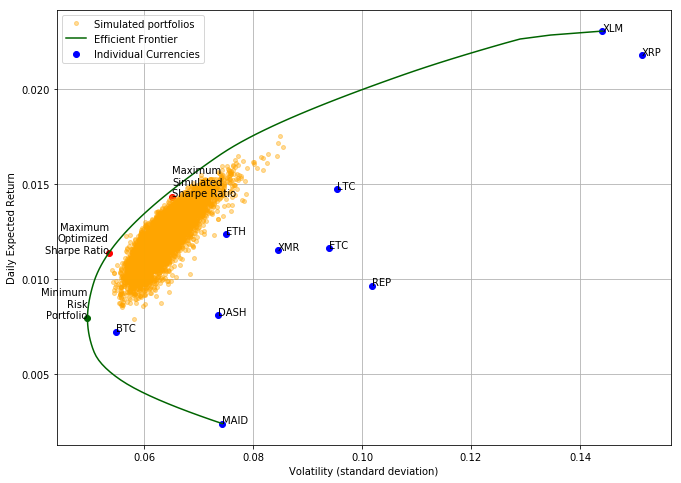
\includegraphics[width=\textwidth]{crypt1}

\subsection{S\&P 500 Stocks}

To validate the cryptocurrency portfolio optimization model, we chose to use the same model on S\&P 500 companies and compare the optimized minimum risk returns to an S\&P 500 index fund. The python optimization model was run on a random subset of 100 companies with daily data since 2015. The model’s results were compared to the index fund's performance over the same period and found our optimized minimum risk portfolio provided very similar return and slightly lower volatility. The minimum risk portfolio had an estimated annual return of 11.6\% and volatility of 0.10, while the index fund had annual return of 11\% and volatility of 0.13. 

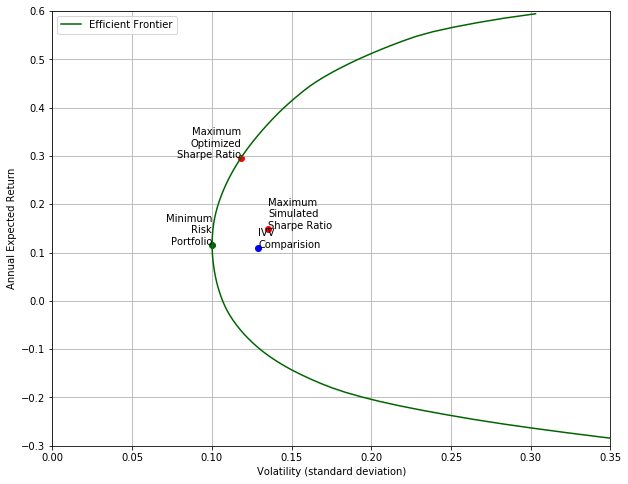
\includegraphics[width=\textwidth]{sp1}
 
\section{Discussion and Conclusions}

Based on the findings from our simulations and optimizations, the portfolio optimization techniques provide a reasonable method to minimize the risk associated with investing in cryptocurrencies. Our results indicate returns of approximately 1\% daily, however, the current state of the cryptocurrency markets make this appear unlikely to hold true, at least in the short-term. The cryptocurrency analysis was based on the past year of data, however, the mean returns and optimized portfolios are likely to significantly change for longer or shorter time periods. For short-term investments, a shorter time period with more granular return data would provide more relevant optimized portfolios, and conversely, long-term investments would most likely benefit from a longer range of data.

To improve our optimization models in future work, we have several proposed ideas to pursue. First, the number of currencies in the optimized portfolio can have a large impact on the results. The number of cryptocurrencies has increased significantly in the past few years, with over 2,300 unique currencies listed by the CryptoCompare API. The analysis for this paper only considered 10 currencies, so including more may lead to optimized portfolios with better performance. Additionally, we may have reason to have a minimum or maximum amount for each held currency, so constraints could be added that may improve performance.

We would also attempt to address issues such as autoregression, asymmetric volatility, skewness, and kurtosis which are challenges to Markowitz’s model we have seen tackled by economists in our research. In regard to the high volatility of cryptocurrencies, we have learned that regularization of the covariance matrix may help improve the accuracy of our estimated variance for the portfolios.

Lastly, we would be interested in exploring the use of neural networks in our optimization models. The research done in this area shows promising results that may lead to significant improvements to the models.

In Summary, portfolio optimization can be used to minimize the risk when investing in volatile financial assets like cryptocurrencies. Building on the time-tested foundations developed by Markowitz and Sharpe, modern optimization techniques will create new and interesting methods of minimizing risk while maximizing gains.

\begin{thebibliography}{1}

\bibitem{copula} Copula (probability theory). (2018, February 23). In \emph{Wikipedia}. Retrieved from
\url{ https://en.wikipedia.org/w/index.php?title=Copula_(probability_theory)&oldid=827164839}

\bibitem{starke} Dr. Thomas Starke, David Edwards, \& Dr. Thomas Wiecki. (2015, March 9). The Efficient Frontier: Markowitz portfolio optimization in Python. Retrieved March 10, 2018, from \url{https://blog.quantopian.com/markowitz-portfolio-optimization-2/}

\bibitem{freitas} Freitas, F. D., De Souza, A. F., \& de Almeida, A. R. (2009). Prediction-based portfolio optimization model using neural networks. \emph{Neurocomputing}, 72(10), 2155–2170. \url{https://doi.org/10.1016/j.neucom.2008.08.019}

\bibitem{garcia} Garcia, D., \& Schweitzer, F. (2015). Social signals and algorithmic trading of Bitcoin. \emph{Royal Society Open Science}, 2(9). \url{https://doi.org/10.1098/rsos.150288}

\bibitem{gregory} Gregory, C., Darby-Dowman, K., \& Mitra, G. (2011). Robust optimization and portfolio selection: The cost of robustness. \emph{European Journal of Operational Research}, 212(2), 417–428. \url{https://doi.org/10.1016/j.ejor.2011.02.015}

\bibitem{hong} Hong, K. (2017). Bitcoin as an alternative investment vehicle. \emph{Information Technology and Management}, 18(4), 265–275. \url{https://doi.org/10.1007/s10799-016-0264-6}

\bibitem{bradford} Investment Portfolio Optimization. (n.d.). Retrieved March 10, 2018, from \url{http://www.bradfordlynch.com/blog/2015/12/04/InvestmentPortfolioOptimization.html}

\bibitem{liu} Liu, Q., Dang, C., \& Huang, T. (2013). A One-Layer Recurrent Neural Network for Real-Time Portfolio Optimization With Probability Criterion. \emph{IEEE Transactions on Cybernetics}, 43(1), 14–23. \url{https://doi.org/10.1109/TSMCB.2012.2198812}

\bibitem{markowitz} Markowitz, H. (1952). Portfolio Selection. \emph{The Journal of Finance}, 7(1), 77–91. \url{https://doi.org/10.2307/2975974}

\bibitem{peng} Peng, Y., Albuquerque, P. H. M., Camboim de Sá, J. M., Padula, A. J. A., \& Montenegro, M. R. (2018). The best of two worlds: Forecasting high frequency volatility for cryptocurrencies and traditional currencies with Support Vector Regression. \emph{Expert Systems with Applications}, 97, 177–192. \url{https://doi.org/10.1016/j.eswa.2017.12.004}

\bibitem{polak} Polak, G. G., Rogers, D. F., \& Sweeney, D. J. (2010). Risk management strategies via minimax portfolio optimization.\emph{ European Journal of Operational Research}, 207(1), 409–419. \url{https://doi.org/10.1016/j.ejor.2010.04.025} 

\bibitem{sharpe66} Sharpe, W. F. (1966). Mutual Fund Performance. \emph{The Journal of Business}, 39(1), 119–138.

\bibitem{sharpe71} Sharpe, W. F. (1971). A Linear Programming Approximation for the General Portfolio Analysis Problem. \emph{Journal of Financial \& Quantitative Analysis}, 6(5), 1263–1275.

\bibitem{xidonas} Xidonas, P., Mavrotas, G., Hassapis, C., \& Zopounidis, C. (2017). Robust multiobjective portfolio optimization: A minimax regret approach. \emph{European Journal of Operational Research}, 262(1), 299–305. \url{https://doi.org/10.1016/j.ejor.2017.03.041}

\bibitem{young} Young, M. R. (1998). A Minimax Portfolio Selection Rule with Linear Programming Solution. Management Science, 44(5), 673–683. \url{https://doi.org/10.1287/mnsc.44.5.673}

\bibitem{zhang04a} Zhang, Y., \& Hua, Y. (2004a). Portfolio Optimization for Multi-stage Capital Investment with Neural Networks. In F.-L. Yin, J. Wang, \& C. Guo (Eds.), Advances in Neural Networks - ISNN 2004 (Vol. 3174, pp. 982–987). Berlin, Heidelberg: Springer Berlin Heidelberg. \url{https://doi.org/10.1007/978-3-540-28648-6_156}

\bibitem{zhang04b} Zhang, Y., \& Hua, Y. (2004b). Portfolio Optimization for Multi-stage Capital Investment with Neural Networks. In Advances in Neural Networks - ISNN 2004 (pp. 982–987). Springer, Berlin, Heidelberg. \url{https://doi.org/10.1007/978-3-540-28648-6_156}

\bibitem{zhao} Zhao, Y., Stasinakis, C., Sermpinis, G., \& Shi, Y. (2018). Neural network copula portfolio optimization for exchange traded funds. Quantitative Finance, 0(0), 1–15. \url{https://doi.org/10.1080/14697688.2017.1414505}


\end{thebibliography}

\section*{Appendix}

\subsection*{ASPE - Markowitz}

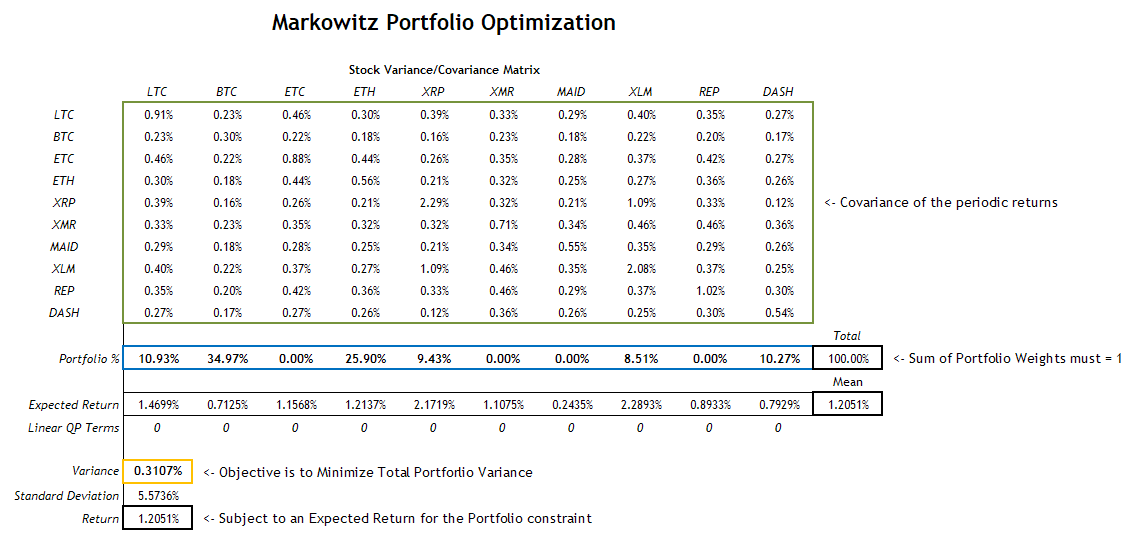
\includegraphics[width=\textwidth]{aspe1}
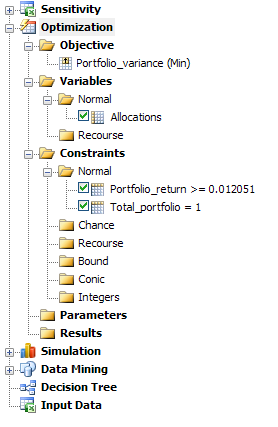
\includegraphics[width=0.4\textwidth]{aspe2}

\subsection*{ASPE - Sharpe}
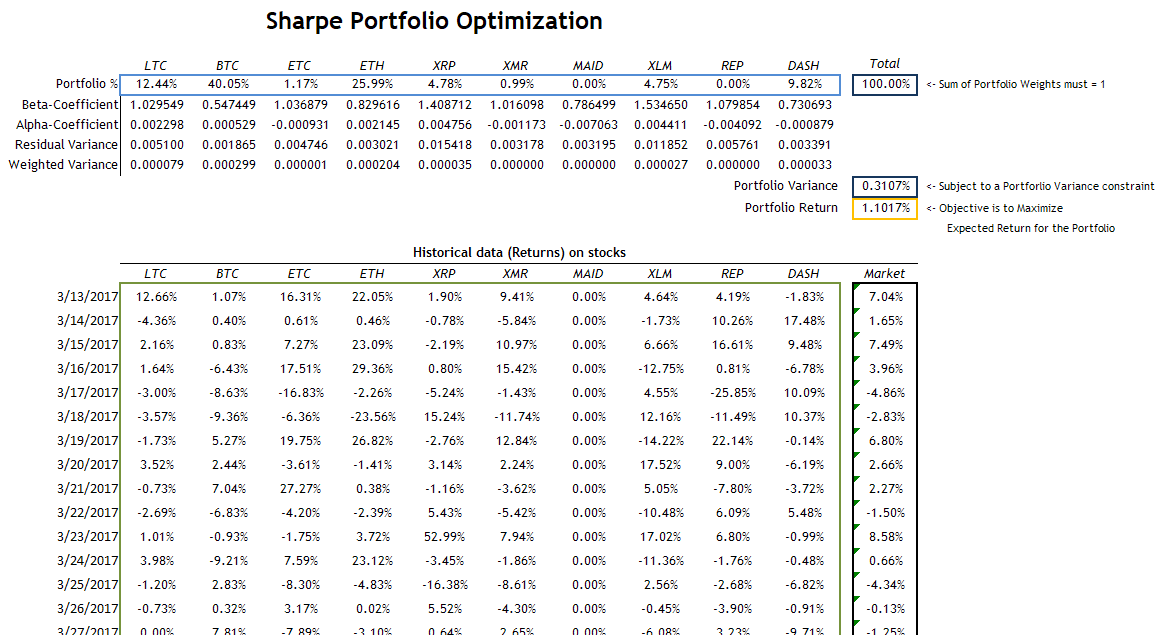
\includegraphics[width=\textwidth]{aspe3}
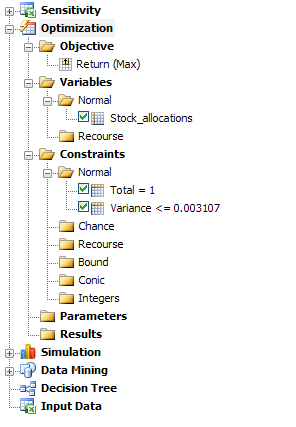
\includegraphics[width=0.4\textwidth]{aspe4}

\subsection*{Python - Cryptocurrencies}
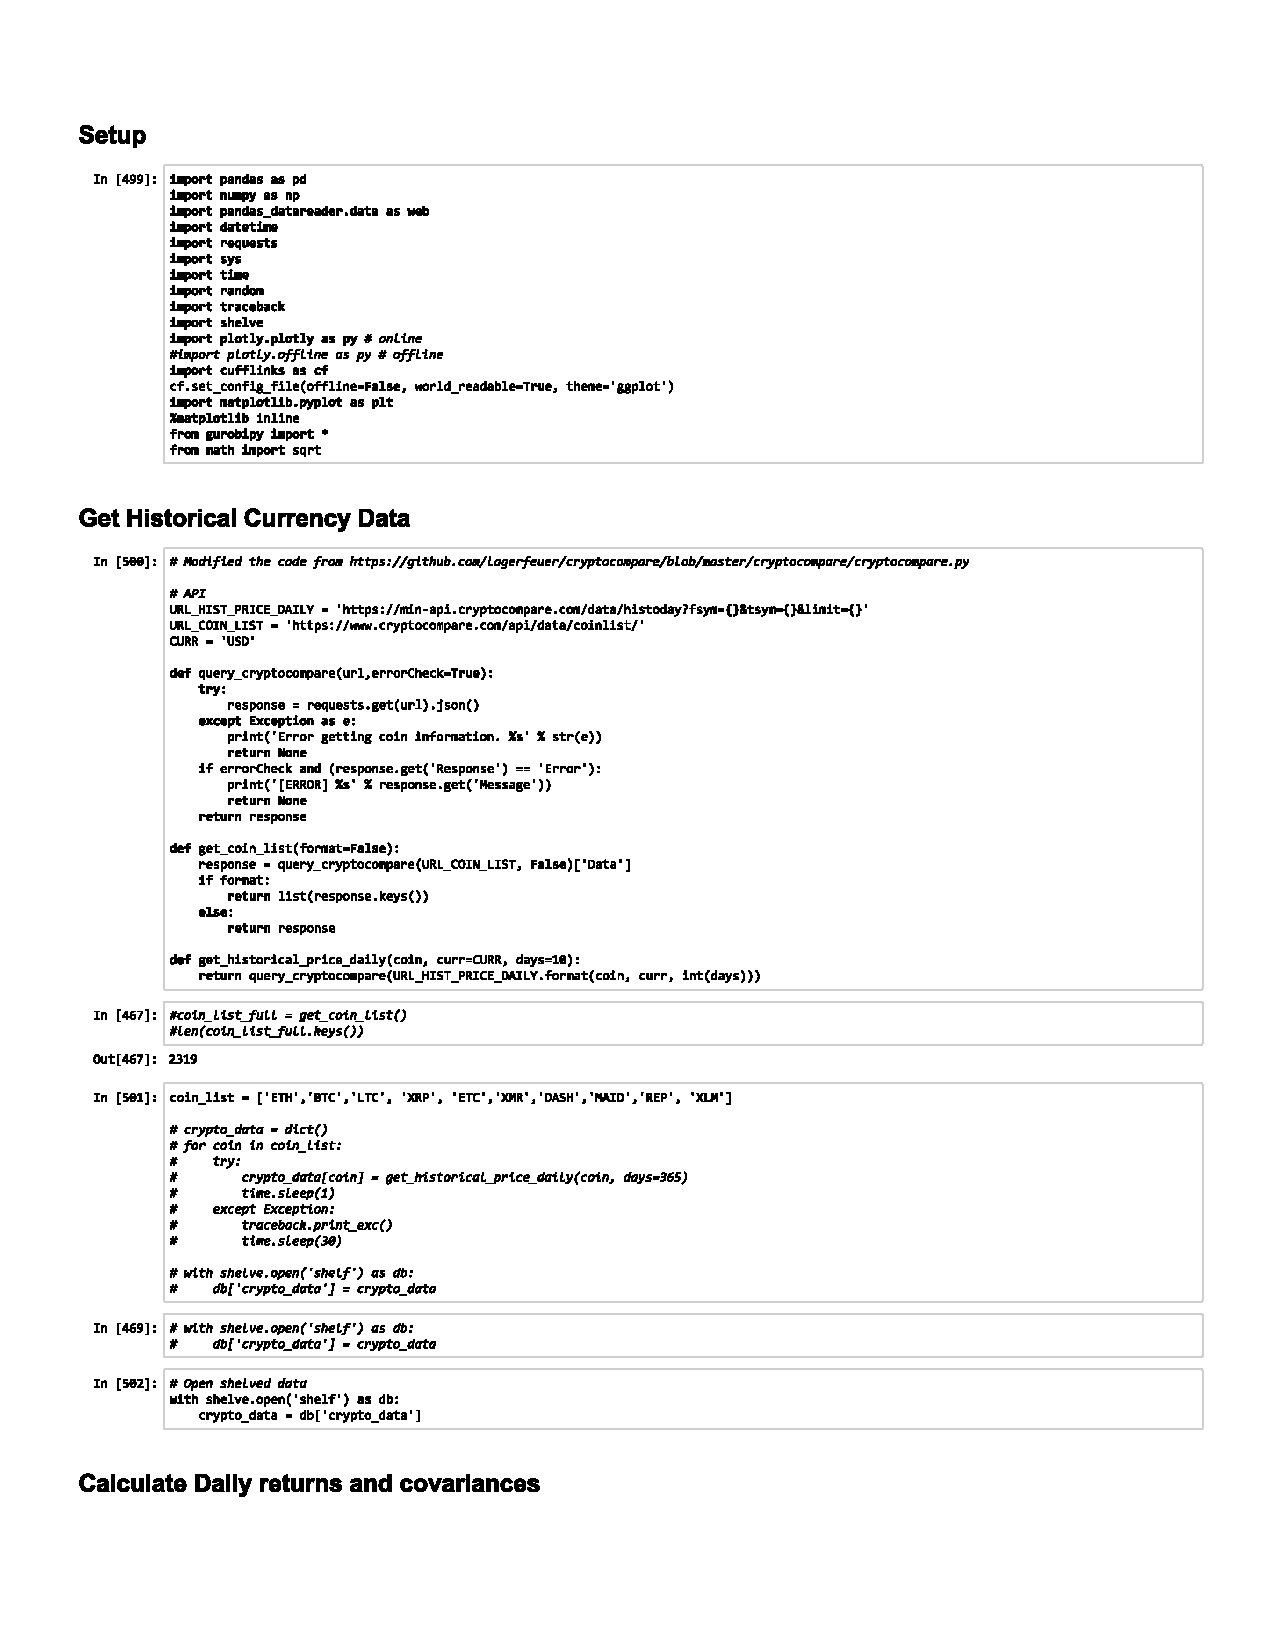
\includepdf[pages=-,scale=.8,pagecommand={}]{crypto_notebook.pdf}

\subsection*{Python - Stocks}
\includepdf[pages=-,scale=.8,pagecommand={}]{stocks_notebook.pdf}




\end{document}
